\documentclass{beamer}


% Use a modern academic theme (e.g., metropolis)
\usetheme{metropolis}
\usecolortheme{default}
\usepackage[T1]{fontenc} % Added for robust font encoding, which helps with symbol rendering like \Letter
\usepackage{graphicx}
\usepackage{booktabs}
\usepackage{amsmath}
\usepackage{hyperref}
\usepackage{bm}
\usepackage{multirow}
\usepackage{subcaption} % For side-by-side figures
\usepackage{textcomp} % For \Letter
\usepackage{colortbl} % For rowcolor in tables
\usepackage{pifont}   % Added for \cmark and \xmark symbols
\usepackage{amssymb}  % Added for \cmark and \xmark symbols, and other math symbols

% Define \cmark and \xmark for use in tables (required by the code but not defined)
\newcommand{\cmark}{\ding{51}}%
\newcommand{\xmark}{\ding{55}}%

% For highlighting
\newcommand{\alertterm}[1]{\alert{\textbf{#1}}}

% fix: \bench undefined; define it as 'Paper2Video'
\newcommand{\bench}{Paper2Video}

% Title and author information
% To include an image on the title page, it's generally recommended to use \titlegraphic
% instead of putting \includegraphics directly into the \title command,
% as some themes might process the \title argument in ways that conflict with graphics commands.
% The \titlegraphic command is sometimes undefined if placed before \title, \author, and \date.
% Moving it after these declarations often resolves the 'Undefined control sequence' error.
\title[Paper2Video]{Paper2Video: Automatic Video Generation from Scientific Papers} % Cleaned title text
\author[Zeyu Zhu, Kevin Q. Lin, Mike Z. Shou]{
  Zeyu Zhu\textsuperscript{*}, Kevin Qinghong Lin\textsuperscript{*}, Mike Zheng Shou ✉ \\ % Original code had '✉' here. The comment stated it was a correction for '\Letter' which caused an error. Keeping the corrected symbol to avoid reintroducing an error.
  {\small Show Lab, National University of Singapore}
}
\date{\today}
\titlegraphic{
\includegraphics[height=0.6cm]{figure/logo_.png}} % Moved the logo definition here to resolve potential error

% Adjust caption font size for better readability in slides
\setbeamerfont{caption}{size=\scriptsize}

% Define colors from source for table
\definecolor{grayblue}{RGB}{170, 180, 230}
\definecolor{lightblue}{RGB}{150, 200, 255}
\definecolor{citecolor}{HTML}{0071bc} % Defined in source for links/ticks



\setbeamerfont{caption}{size=\scriptsize}
\begin{document}
\begin{frame}
  \titlepage
\end{frame}
\begin{frame}{Motivation}
  % Corresponds to source text Section 1
  \begin{figure}
      \centering
      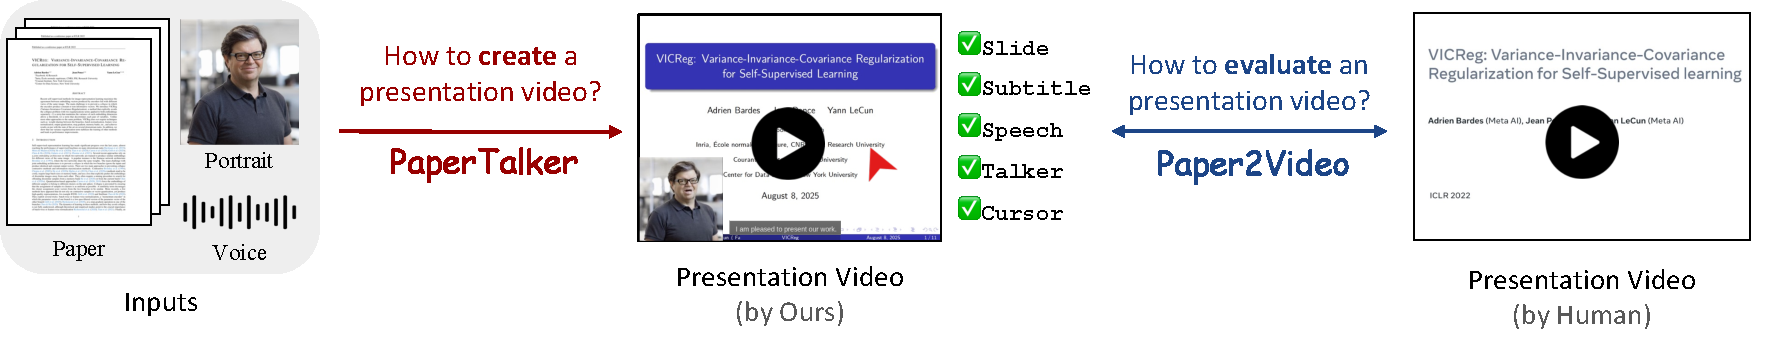
\includegraphics[width=0.9\linewidth]{figure/teaser.pdf}
      \vspace{-1\baselineskip}
      \caption{Motivation: Automating academic presentation video generation.}
      \label{fig:teaser_motivation}
  \end{figure}
  \vspace{-1\baselineskip}
 \begin{block}{\small Problem Statement}
 \footnotesize
 \footnotesize
  \begin{itemize}
    \item \textbf{Academic presentation videos} are essential for research dissemination.
    \item \alertterm{Producing them is highly labor-intensive}: involves slide design, recording, subtitling, editing.
    \item \alertterm{Challenge:} Presentation video generation is a complex, multi-modal, long-context task with no existing benchmarks or tailored metrics.
  \end{itemize}
  </block>
  \begin{block}{\small Key Questions}
    \footnotesize
    \footnotesize
    \begin{itemize}
      \item What defines a \alertterm{good academic presentation video}?
      \item How to \alertterm{automatically generate} such a video from a research paper?
    \end{itemize}
  </block>
\end{frame}
\begin{frame}{Related Work: Status \& Challenges} % Corrected: Changed '&' to '\&' in the frame title to escape the special character.
  % Corresponds to source text Section 2
  \begin{block}{\small Overview of Existing Solutions}
   \footnotesize
    \small
    \begin{itemize}
      \item \alertterm{Natural Video Generation}: Advances in diffusion models, but limited by short durations, multi-shot, and complex conditioning.
      \item \alertterm{Multi-Agent Frameworks}: PPTAgent, PresentAgent focus on slides/narration but lack personalization, academic formality, and comprehensive multi-modal alignment.
      \item \alertterm{Core Gap}: No existing solution fully addresses the specific challenges of academic presentation video generation.
    \end{itemize}
  </block>
  \begin{table}[ht]
    \centering
    \tiny % Using tiny to fit the table
    \caption{\textbf{Comparison of \bench~with existing benchmarks.} (Excerpt from original Table 1 in Section 2)}
    \label{tab:related_work_comparison}
    \setlength{\tabcolsep}{2pt} % Reduce column separation
    \begin{tabular}{@{}lccccccc@{}}
      \toprule
      \multirow{2}{*}{Benchmarks} &
      \multirow{2}{*}{Inputs} &
      \multirow{2}{*}{Outputs} &
      \multirow{2}{*}{Subtitle} &
      \multirow{2}{*}{Slides} &
      \multirow{2}{*}{Cursor} &
      \multicolumn{2}{c}{Speaker} \\
      \cmidrule(lr){7-8}
       & & & & & & Face & Voice \\
      \midrule
      \multicolumn{8}{c}{{\textcolor[RGB]{105, 105, 105}{\textit{Natural Video Generation}}}}  \\
      VBench~\cite{vbench} & Text & Short Vid. & \xmark & \xmark & \xmark & \xmark & \xmark \\
      MovieBench~\cite{wu2025moviebench} & Text\&Audio\&Image & Long Vid. & \textcolor{citecolor}{\cmark} & \xmark & \xmark & \textcolor{citecolor}{\cmark} & \textcolor{citecolor}{\cmark} \\
      \midrule
      \multicolumn{8}{c}{{\textcolor[RGB]{105, 105, 105}{\textit{Multimodal Agent for Research}}}}  \\
      PPTAgent~\cite{zheng2025pptagent} & Doc.\&Template & Slide & \xmark & \textcolor{citecolor}{\cmark} & \xmark & \xmark & \xmark \\
      PresentAgent~\cite{shi2025pptagent} & Doc.\&Template & Audio\&Long Vid. & \textcolor{citecolor}{\cmark} & \textcolor{citecolor}{\cmark} & \xmark & \xmark & \xmark \\
      \bench~(Ours) & Paper\&Image\&Audio & Audio\&Long Vid. & \textcolor{citecolor}{\cmark} & \textcolor{citecolor}{\cmark} & \textcolor{citecolor}{\cmark} & \textcolor{citecolor}{\cmark} & \textcolor{citecolor}{\cmark} \\
      \bottomrule
    \end{tabular}
  \end{table}
  \vspace{-0.5\baselineskip}
  \begin{block}{\small Our Differentiation}
   \footnotesize
    \small
    \begin{itemize}
      \item Addresses multi-modal, long-context, multi-task challenges in academic video generation.
      \item Introduces \alertterm{full control over all presentation elements} (slides, subtitles, cursor, personalized presenter).
    \end{itemize}
  </block>
\end{frame}
\begin{frame}{\bench~Benchmark \& Metrics}
  % Corresponds to source text Section 3
  \begin{columns}
    \begin{column}{0.5\textwidth}
      \begin{figure}
        \centering
        \begin{subfigure}[b]{0.48\textwidth}
          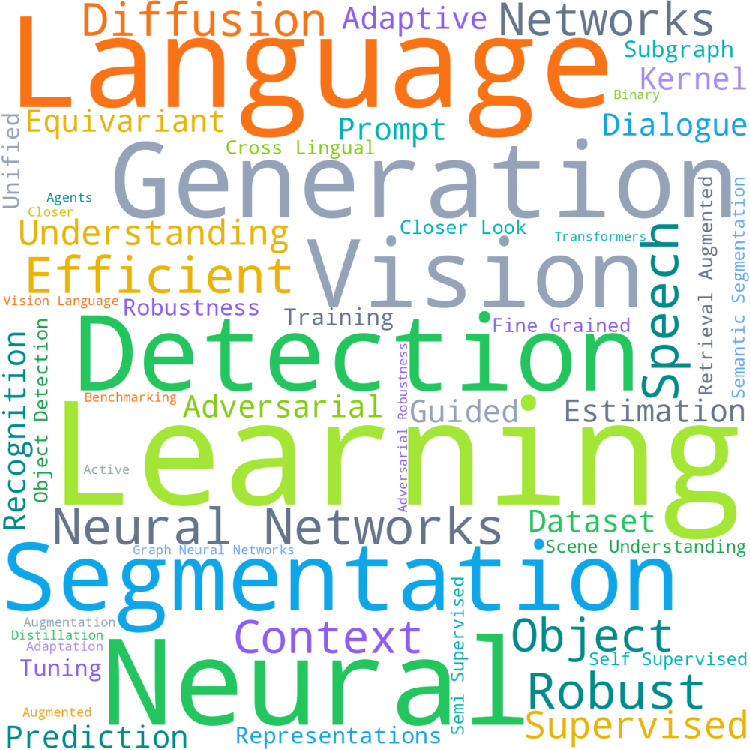
\includegraphics[width=\linewidth]{figure/paper_topics_wordcloud.pdf}
          \caption{Paper topics}
        \end{subfigure}
        \hfill
        \begin{subfigure}[b]{0.48\textwidth}
          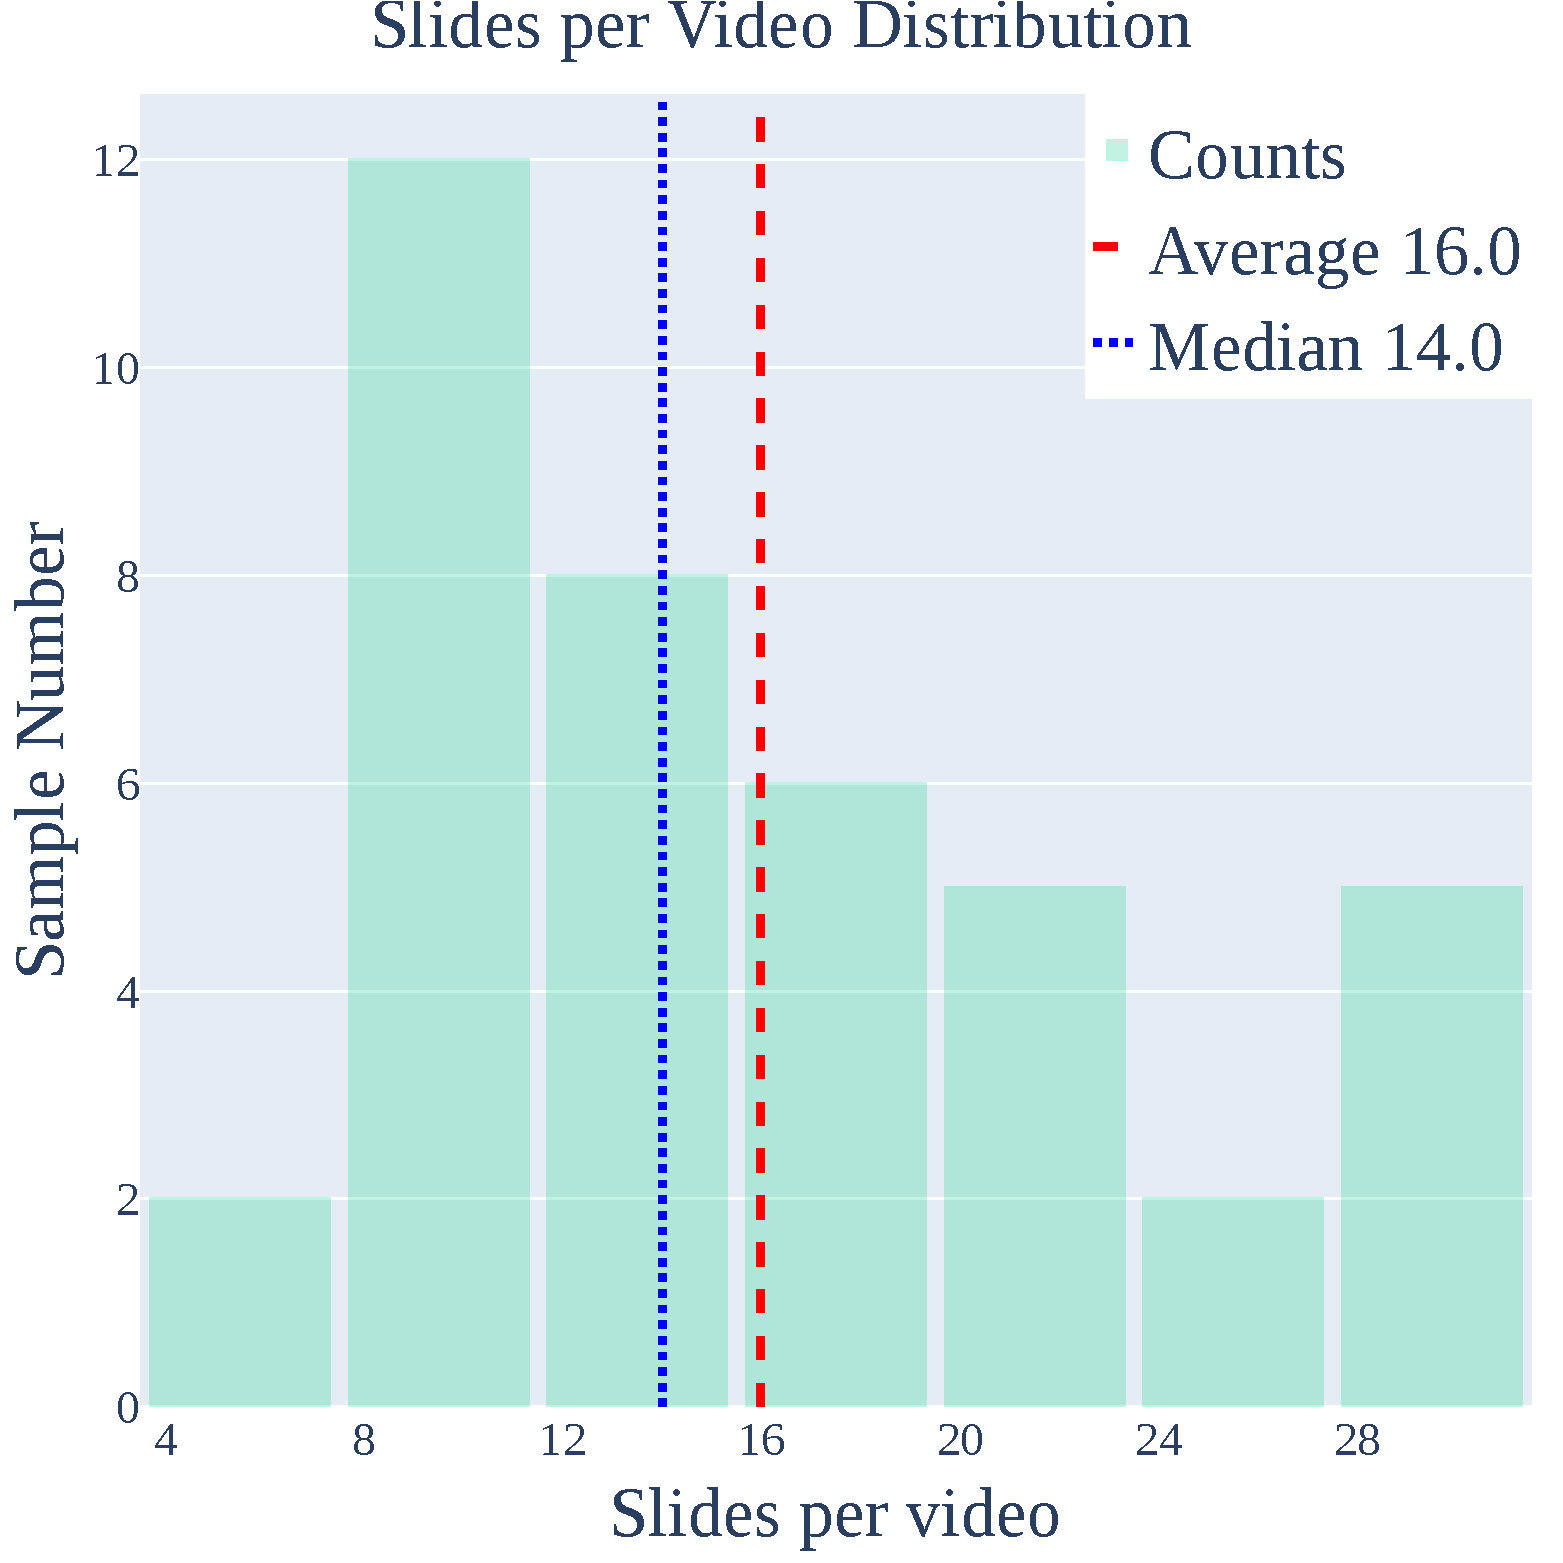
\includegraphics[width=\linewidth]{figure/slides_count_hist.pdf}
          \caption{Slides count}
        \end{subfigure}
        \begin{subfigure}[b]{0.95\textwidth}
          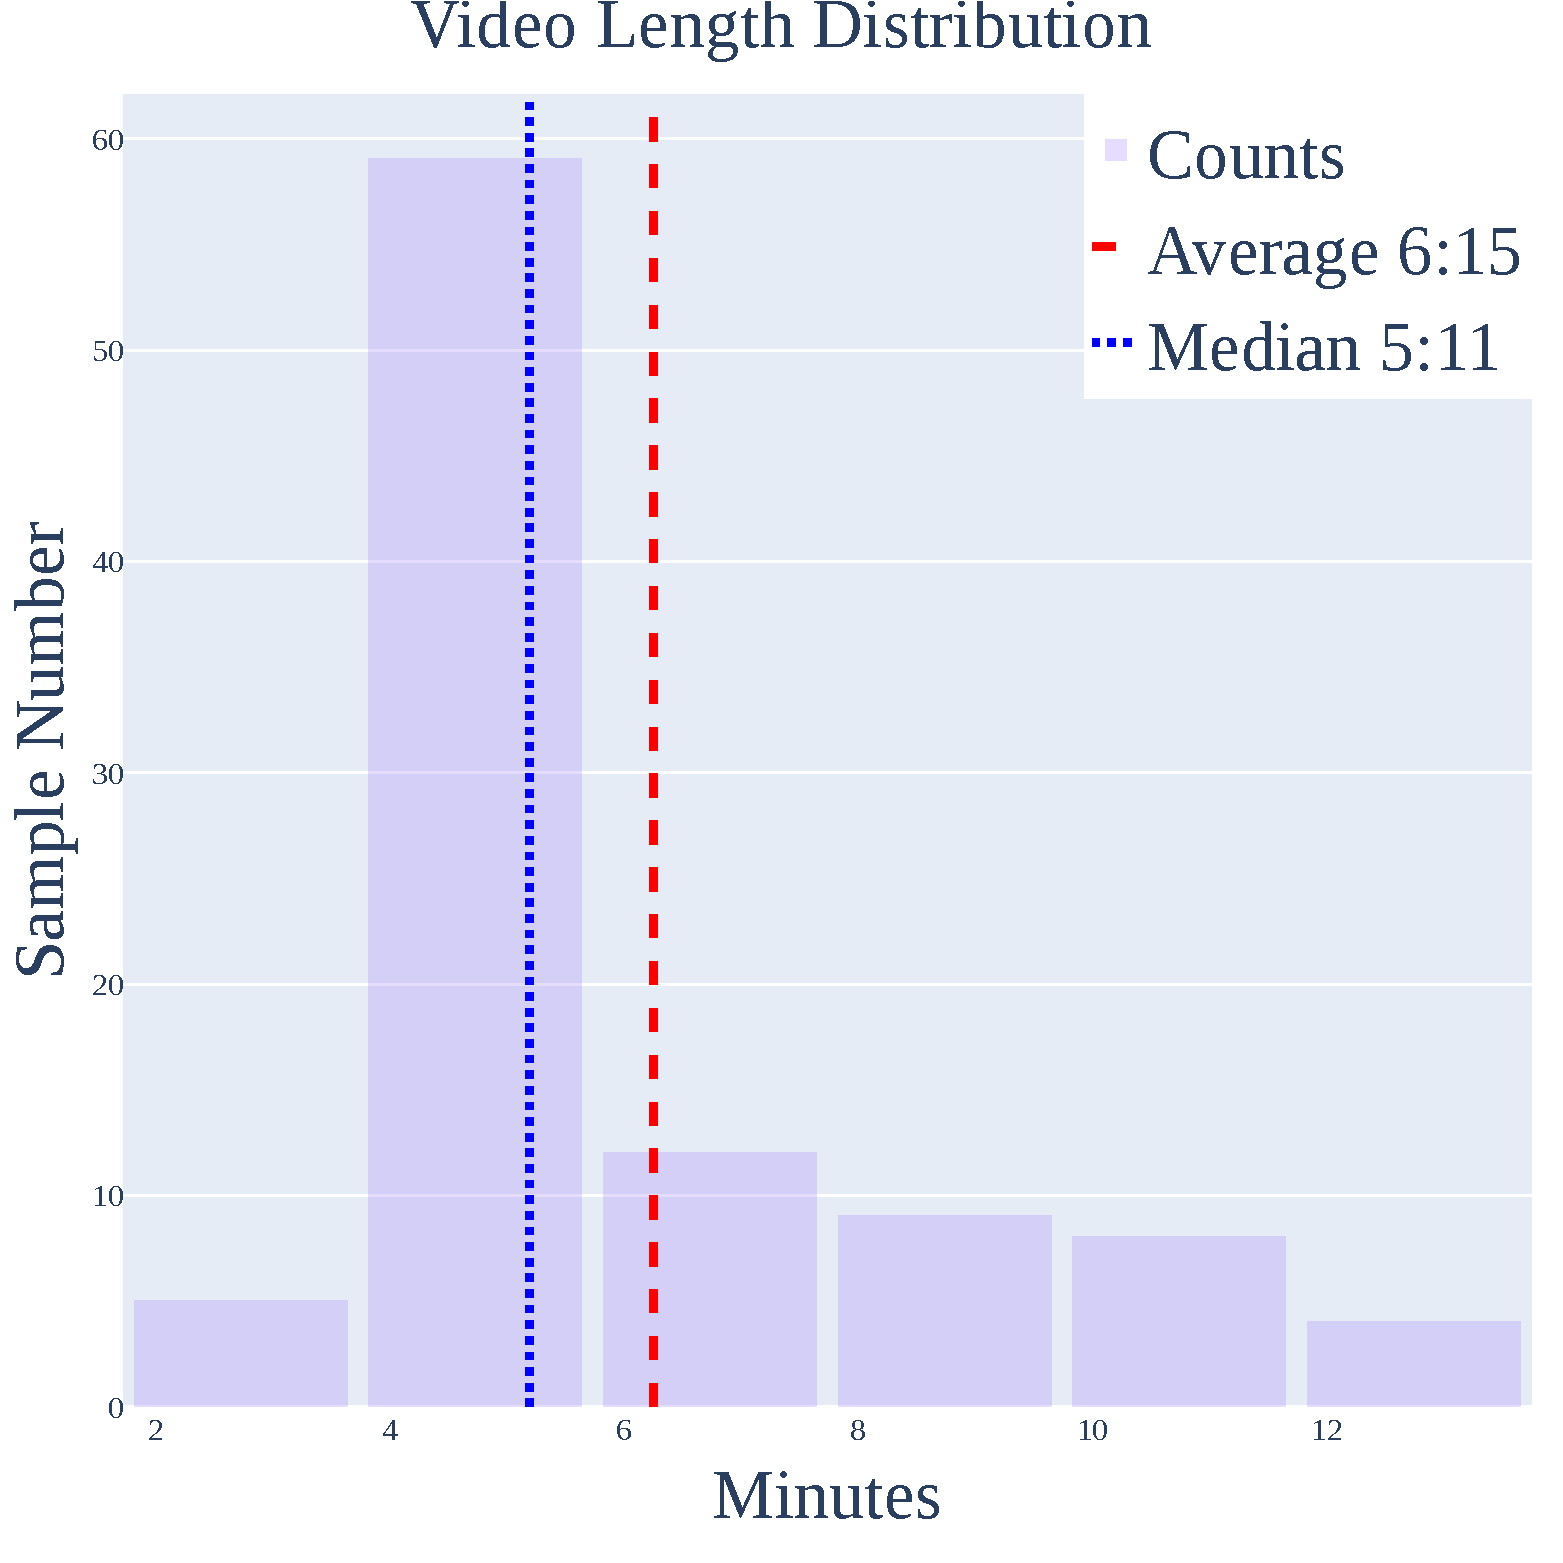
\includegraphics[width=\linewidth]{figure/video_length_hist.pdf}
          \caption{Video lengths}
        \end{subfigure}
        \caption{Statistics of \alertterm{\bench} benchmark.}
        \label{fig:stat_benchmark}
      \end{figure}
    \end{column}
    \begin{column}{0.5\textwidth}
      \vspace{-2.5\baselineskip}
      \begin{block}{The \alertterm{\bench} Benchmark}
       \footnotesize
        \small
        \begin{itemize}
          \item First benchmark with \alertterm{101 research papers}, paired with author-created videos, slides, and metadata.
          \item Curated from diverse AI conferences (\alertterm{ML, CV, NLP}).
          \item Averages 13.3K words, 44.7 figures, 16 slides, and 6 minutes per video.
        \end{itemize}
      \end{block}
      \vspace{-0.5\baselineskip}
      \begin{block}{Evaluation Metrics}
       \footnotesize
        \small
        \begin{itemize}
          \item \alertterm{Meta Similarity}: Alignment to human-created content.
          \item \alertterm{PresentArena}: Pairwise quality contest via VideoLLM.
          \item \alertterm{PresentQuiz}: Information coverage via video QA.
          \item \alertterm{IP Memory}: Author/work recall after watching the video.
        \end{itemize}
      \end{block}
      \begin{figure}
        \centering
        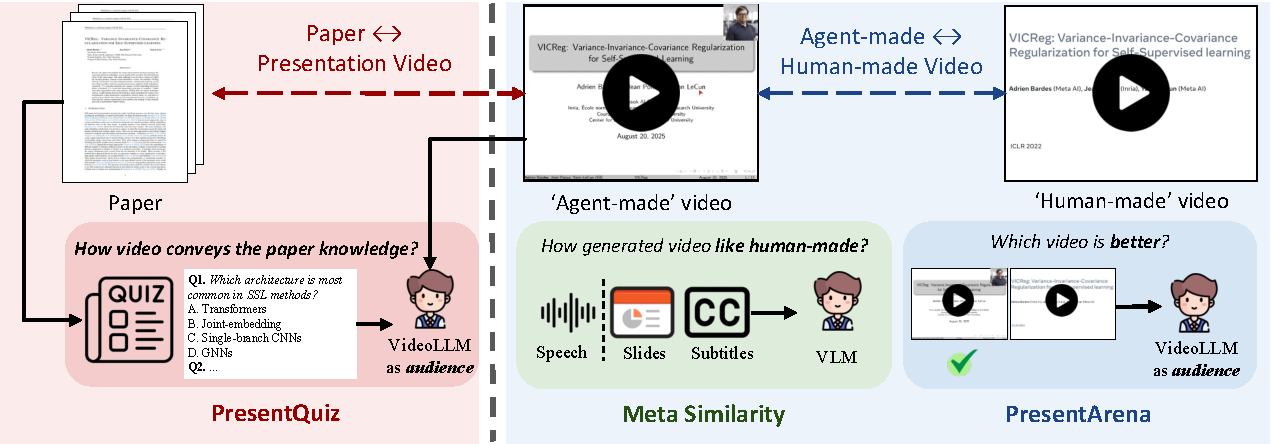
\includegraphics[width=0.9\linewidth]{figure/eval.pdf}
        \vspace{-1.5\baselineskip}
        \caption{Overview of \alertterm{evaluation metrics}.}
        \label{fig:eval_overview}
      \end{figure}
    \end{column}
  \end{columns}
</frame>

% Corresponds to the source text Section 4: Method
\begin{frame}{Method Overview: PaperTalker Agent}
  % Corresponds to source text Section 4
  \begin{figure}
    \centering
    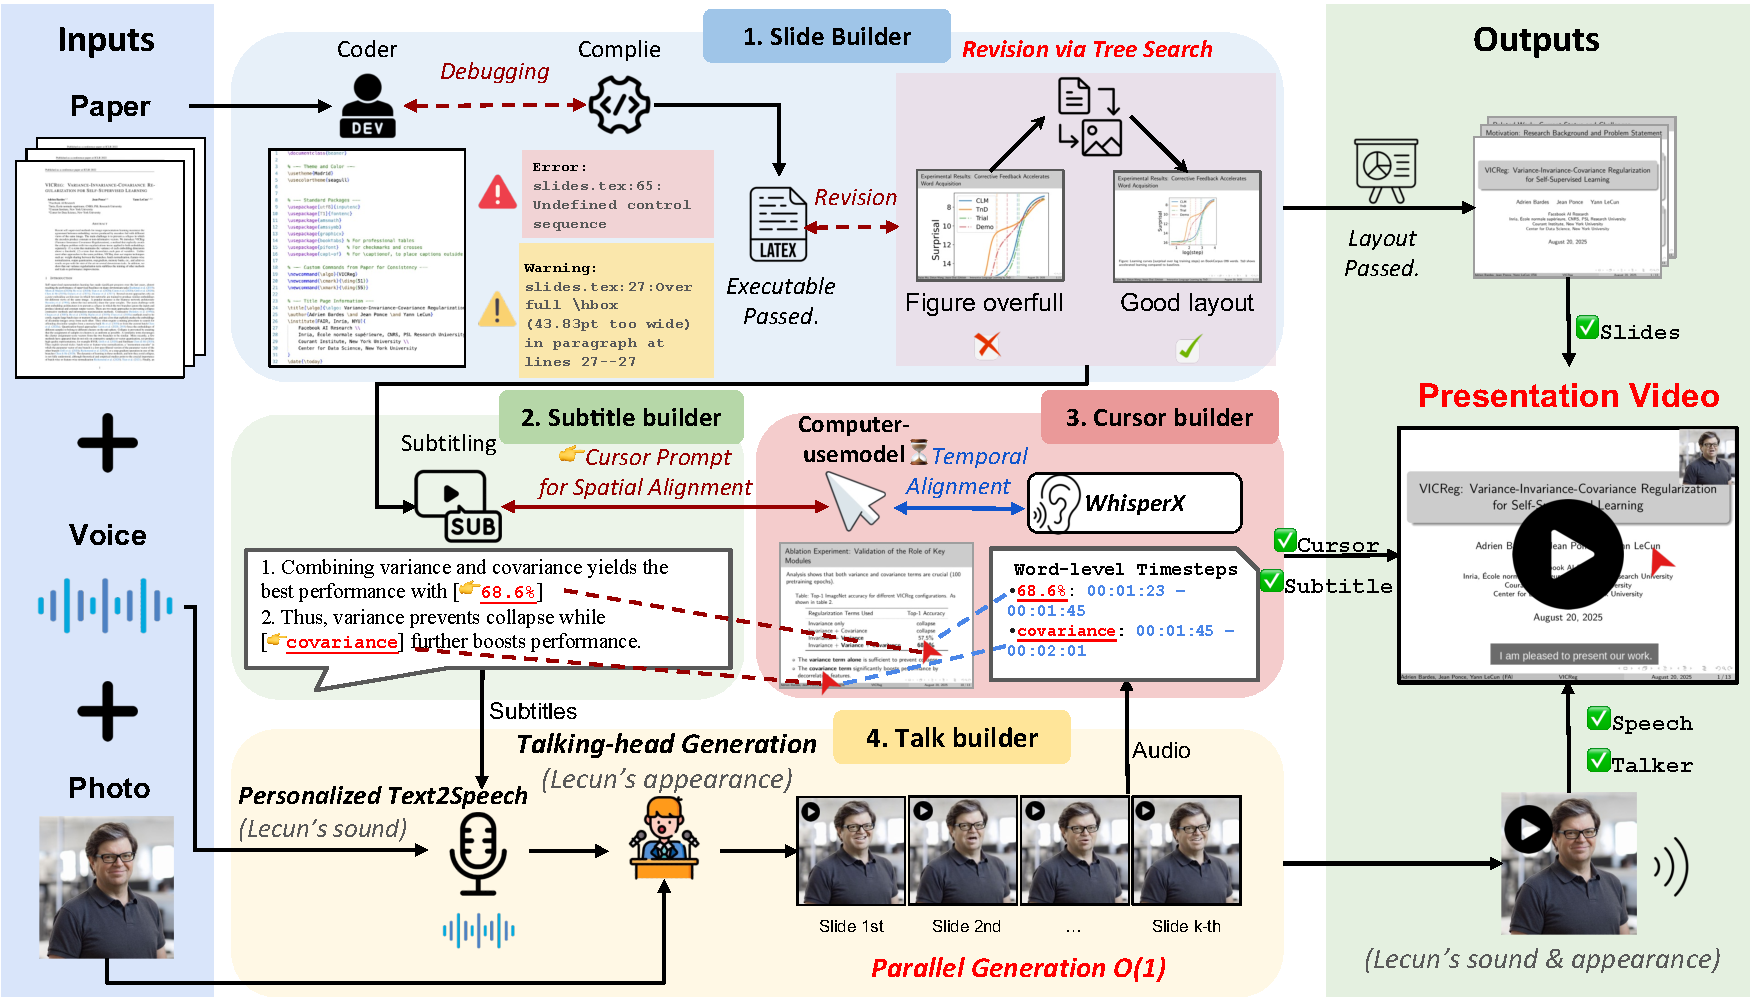
\includegraphics[width=0.8\textwidth]{figure/method.pdf}
    \vspace{-1\baselineskip}
    \caption{Overall pipeline of \alertterm{PaperTalker} for presentation video generation.}
    \label{fig:method_overview}
  \end{figure}
  \vspace{-1 \baselineskip}
  \begin{block}{Key Modules of \alertterm{PaperTalker}}
   \footnotesize
    \small
    \begin{itemize}
      \item \alertterm{Slide Builder}: Generates \LaTeX~Beamer slides, with visual layout refinement.
      \item \alertterm{Subtitle \& Cursor Builder}: Produces subtitles and aligns them with spatial-grounded cursor.
      \item \alertterm{Talker Builder}: Synthesizes personalized speech and renders a talking-head presenter.
      \item Supports \alertterm{slide-wise parallelization} for efficiency.
    \end{itemize}
  \end{block}
</frame>

% Corresponds to the source text Section 4.1: Slide Builder
\begin{frame}{Method: Slide Builder / Layout Refinement}
  % Corresponds to source text Section 4.1
  \begin{columns}
    \begin{column}{0.5\textwidth}
      \begin{block}{\small Core Ideas}
       \footnotesize
        \small
        \begin{itemize}
          \item \alertterm{Slides} created directly from paper's \LaTeX~source using Beamer for formal, academic layouts.
          \item Uses compiler feedback to iteratively fix issues (grammar, content coverage).
          \item Addresses LLM insensitivity to fine-grained numeric adjustments in layout.
        \end{itemize}
      \end{block}
    \end{column}
    \begin{column}{0.5\textwidth}
      \begin{figure}
        \centering
        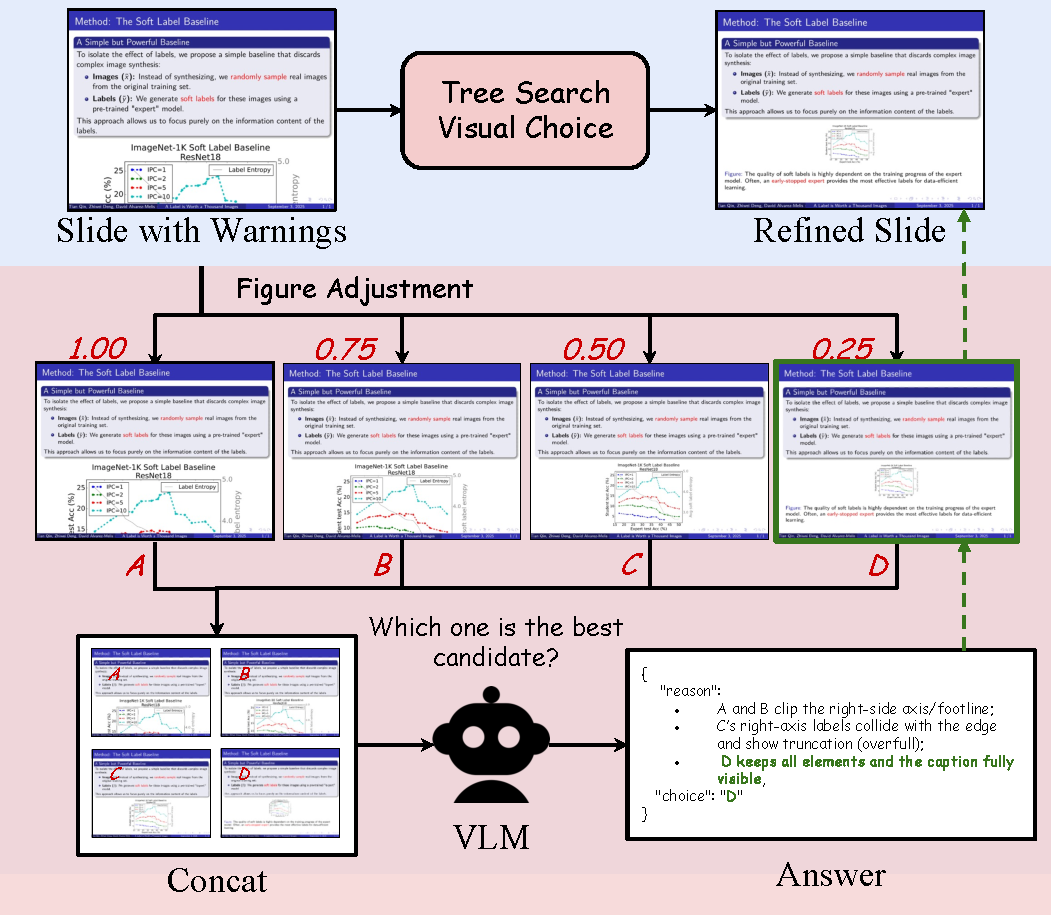
\includegraphics[width=0.95\linewidth]{figure/tree_search.pdf}
        \vspace{-1\baselineskip}
        \caption{\alertterm{Tree Search Visual Choice:} Visual refinement to resolve overfull/overflow slides.}
        \label{fig:tree_search_method}
      \end{figure}
      \vspace{-1\baselineskip}
      \begin{block}{\small \alertterm{Tree Search Visual Choice}}
       \footnotesize
        \small
        \begin{itemize}
          \item Novel technique for fine-grained layout optimization.
          \item Explores rule-based parameter variants (font, figure scales).
          \item Renders variants to images.
          \item A VLM selects the best layout based on visual quality.
        \end{itemize}
      \end{block}
    \end{column}
  \end{columns}
</frame>

% Corresponds to the source text Section 4.2: Subtitle Builder, Section 4.4: Cursor Builder, Section 4.3: Talker Builder
\begin{frame}{Method: Subtitle, Cursor \& Talker Builders}
  % Corresponds to source text Section 4.2, 4.3, 4.4
  \begin{columns}
    \begin{column}{0.55\textwidth}
      \begin{block}{\small Subtitle \& Cursor Builder}
       \footnotesize
        \small
        \begin{itemize}
          \item Subtitles generated per slide using a VLM to align content.
          \item \alertterm{Visual Focus Prompts} direct the cursor to key content.
          \item \alertterm{Cursor spatial-temporal alignment}:
            \begin{itemize}
              \item UI-TARS for spatial grounding (position).
              \item WhisperX for temporal alignment (timing with narration).
            \end{itemize}
          \item \alertterm{Benefit}: Enhanced audience guidance and accessibility.
        \end{itemize}
      \end{block}
      \vspace{-0.5\baselineskip}
      \begin{block}{\small Talker Builder}
       \footnotesize
        \small
        \begin{itemize}
          \item Personalized speech synthesis using author voice sample (\alertterm{F5-TTS}).
          \item Realistic talking-head generated with author portrait (\alertterm{FantasyTalking, Hallo2}).
          \alertterm{Parallel per-slide synthesis}: Dramatically speeds up video generation by processing slides independently.
        \end{itemize}
      \end{block}
    \end{column}
    \begin{column}{0.45\textwidth}
      \begin{figure}
        \centering
        
\includegraphics[width=0.8\linewidth]{figure/presenter.png}
        \vspace{-1\baselineskip}
        \caption{Personalized \alertterm{talking-head} presenter output.}
        \label{fig:presenter_method}
      \end{figure}
    \end{column}
  \end{columns}
</frame>

% Corresponds to the source text Section 5.1: Baseline and Settings
\begin{frame}{Experimental Settings}
  % Corresponds to source text Section 5.1
  \begin{block}{\small Baselines}
   \footnotesize
    \small
    \begin{itemize}
      \item \alertterm{End-to-end video generation}: Veo3, Wan2.2 (natural video generation models).
      \item \alertterm{Multi-agent methods}: PresentAgent (combines slide gen with TTS).
      \item \alertterm{Human-created presentations} for direct comparison.
    \end{itemize}
  \end{block}
  \vspace{-0.5\baselineskip}
  \begin{block}{\small Dataset}
   \footnotesize
    \small
    \begin{itemize}
      \item \alertterm{Paper2Video benchmark}: 101 paper/video pairs with author-recorded presentations, slides, and speaker metadata.
    \end{itemize}
  \end{block}
  \vspace{-0.5\baselineskip}
  \begin{block}{\small Resources}
   \footnotesize
    \small
    \begin{itemize}
      \item \alertterm{Hardware}: 8$\times$ NVIDIA RTX A6000 GPUs.
      \item \alertterm{LLM/VLMs}: All methods evaluated using Gemini-2.5-Flash (VideoLLM) and GPT-4.1 (VLM).
    \end{itemize}
  \end{block}
</frame>

% Corresponds to the source text Section 5.2: Main Results
\begin{frame}{Experimental Results: Main}
  % Corresponds to source text Section 5.2
  \begin{table}[ht]
    \centering
    \tiny % Using tiny to fit the table
    \caption{\textbf{Main Evaluation Results}. $\text{PaperTalker}^{*}$ is without presenter and cursor.}
    \label{tab:main_result_exp}
    \setlength{\tabcolsep}{3pt} % Reduce column separation
    \begin{tabular}{l c c c c c c c}
      \toprule
      \multirow{2}{*}{Method} & \multicolumn{2}{c}{Similarity$\uparrow$} & \multirow{2}{*}{Arena$\uparrow$} & \multicolumn{2}{c}{PresentQuiz Acc.$\uparrow$} & \multirow{2}{*}{IP Memory$\uparrow$} & \multirow{2}{*}{Avg. Dur.(s)}\\
      \cmidrule(lr){2-3}\cmidrule(lr){5-6}
      & Speech & Content & & Detail & Under.\\
      \midrule
      HumanMade & \alertterm{1.00} & \alertterm{5.00}  & \alertterm{50.0\%}  & 0.738  & 0.908  & - & 375.15\\
      \midrule
      Wan2.2~\cite{wan} & NA & NA & 1.1\% & 0.251 & 0.551 & 11.5\% & 4.00\\
      Veo3~\cite{deepmind2025veo3} & 0.133 & NA & 1.2\% & 0.367 & 0.585 & 31.3\% & 8.00\\
      PresentAgent~\cite{shi2025pptagent} & 0.045 & 1.47 & 2.0\% & 0.548 & 0.654 & 12.5\% & 430.20\\
      $\text{PaperTalker}^{*}$ & \underline{0.646} & \underline{1.97} & 15.2\% & \underline{0.835}  & \underline{0.949} & \underline{37.5\%} & 234.36 \\
      PaperTalker & \underline{0.646} & \underline{1.97} & \underline{17.0}\% & \textbf{0.842}  & \textbf{0.951} & \textbf{50.0\%} & 234.36\\
      \bottomrule
    \end{tabular}
  \end{table}
  \vspace{0.1cm}
  \begin{columns}
    \begin{column}{0.5\linewidth}
      \centering
      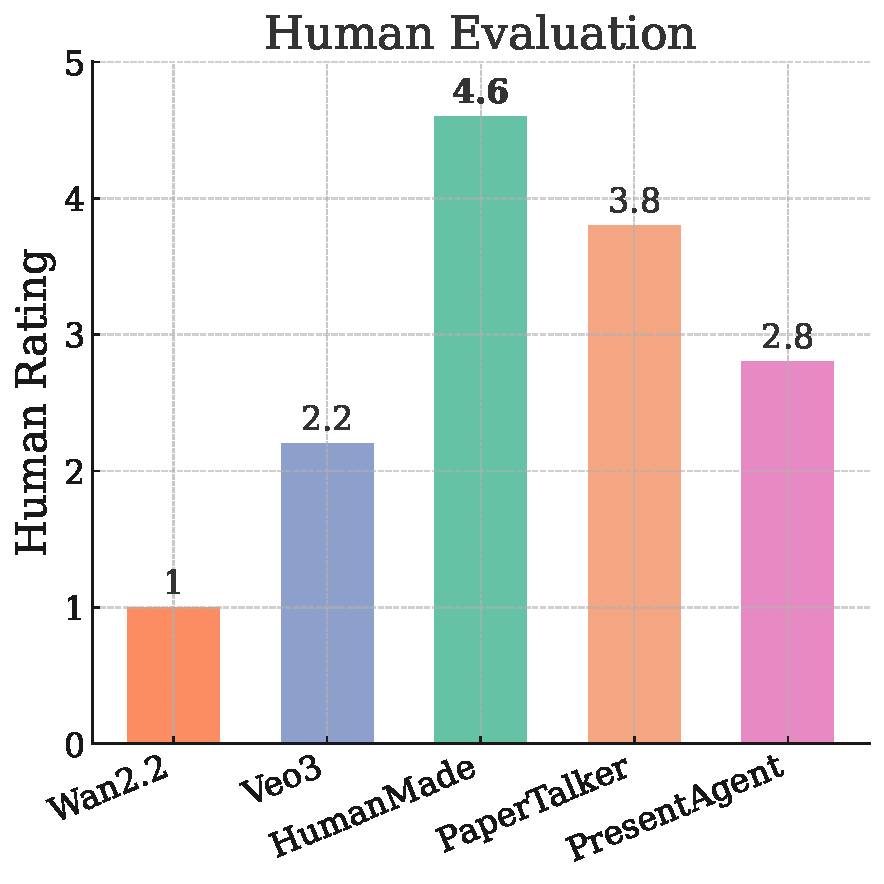
\includegraphics[width=0.7\linewidth]{figure/human_evaluation_bar.pdf}
      \vspace{-1\baselineskip}
      \captionof{figure}{\small Human evaluation: Preference scores.}
      \label{fig:human_eval_bar}
    \end{column}%
    \hfill
    \begin{column}{0.45\linewidth}
      \small
      \begin{itemize}
        \item \alertterm{PaperTalker} outperforms all baselines in automatic metrics (Meta Sim., Arena, Quiz, IP Mem.).
        \item \alertterm{Comparable to HumanMade}: Achieves highest scores across multiple categories, close to human performance.
        \item Human evaluation shows \alertterm{PaperTalker} is consistently preferred over baselines.
        \item Adding presenter video boosts engagement and quality preference by 10\% (Arena).
      \end{itemize}
    \end{column}
  \end{columns}
</frame>

% Corresponds to the source text Section 5.2: Qualitative Analysis (for efficiency table) and Section 5.3: Key Ablations
\begin{frame}{Ablation Experiment \& Efficiency}
  % Corresponds to the source text Section 5.2 (for cost table), Section 5.3 (for ablations)
  \begin{columns}[T] % T=top aligned
    \begin{column}{0.5\textwidth}
      \begin{table} % Removed [H] as 'float' package is not loaded and Beamer handles floats differently.
        \centering
        \small
        \setlength{\tabcolsep}{3pt}
        \caption{\textbf{Generation cost for each method.}}
        \label{table:cost_exp}
        \begin{tabular}{lccc}
          \toprule
          Method & Token (K)$\downarrow$ & Time (min.)$\downarrow$ & Cost (\$)$\downarrow$ \\
          \midrule
          Veo3~\cite{deepmind2025veo3} & NA & \textbf{0.4} & 1.667 \\
          Wan2.2~\cite{wan} & NA & 8.1 & 0.280 \\
          \midrule
          PresentAgent~\cite{shi2025pptagent} & 241 & 39.5 & 0.003  \\
          PaperTalker (w/o Talker) & \textbf{62} & 15.6 & \textbf{0.001}\\
          \midrule
          PaperTalker (w/o Par.) & \textbf{62} & 287.2 & \textbf{0.001}\\
          PaperTalker & \textbf{62} & 48.1 \textbf{(\alertterm{6$\times$})} & \textbf{0.001} \\
          \bottomrule
        \end{tabular}
      \end{table}
      \vspace{-0.3\baselineskip}
      \textbf{Efficiency Highlights:}
      \begin{itemize}
        \item \textbf{Speed vs. PresentAgent:} 39.5 $\rightarrow$ 15.6 min (2.5$\times$ faster).
        \item \textbf{Parallel Generation:} 287.2 $\rightarrow$ 48.1 min (\textbf{6$\times$ speedup}).
        \item \textbf{Lowest Cost:} Only \$0.001, cheapest among all methods.
      \end{itemize}
    \end{column}

    \begin{column}{0.5\textwidth}
      \begin{block}{\small \alertterm{Ablation Study}}
       \footnotesize
        \small
        \begin{itemize}
          \item \textbf{Cursor Highlight}: Markedly improves content localization (QA acc. rises from 8\% to 63\%).
          \item \textbf{Slide Quality}: Tree search refinement fixes layout issues and improves coherence.
        \end{itemize}
      \end{block}
      \vspace{-0.5\baselineskip}
      \centering
      \tiny
      \captionof{table}{\textbf{Ablation study on cursor.}}
      \label{table:cursor_exp}
      \begin{tabular}{lc}
        \toprule
        Method & Accuracy$\uparrow$ \\
        \midrule
        PaperTalker (w/o Cursor) & 0.084 \\
        PaperTalker & \textbf{0.633} \\
        \bottomrule
      \end{tabular}
      \vspace{0.5\baselineskip}
      \captionof{table}{\textbf{Evaluation result on slide quality.}}
      \label{tab:slide_quality_exp}
      \begin{tabular}{lccc}
        \toprule
        Method & Content ($\uparrow$) & Design ($\uparrow$) & Coherence ($\uparrow$) \\
        \midrule
        HumanMade & \textbf{4.43} & \textbf{2.85} & 2.73 \\
        \midrule
        $\text{PPTAgent}_\text{Qwen7B}$ & 3.43 & 1.57 & 1.29 \\
        $\text{PaperTalker}_\text{Qwen7B}$ & 4.00 & 2.53 & \underline{3.11} \\
        \midrule
        $\text{PPTAgent}_\text{GPT4.1}$ & 4.07 & 2.02 & 2.06 \\
        $\text{PaperTalker}_\text{GPT4.1}$(w/o TS) & 4.33 & \underline{2.73} & \textbf{3.84} \\
        $\text{PaperTalker}_\text{GPT4.1}$ & \underline{4.34} & \textbf{2.85} & \textbf{3.84} \\
        \bottomrule
      \end{tabular}
    \end{column}
  \end{columns}
</frame>

% Corresponds to the source text Section 5.2: Qualitative Analysis, and Appendix: Results of Tree Search Visual Choice
\begin{frame}{Visualization Comparison}
  % Corresponds to source text Section 5.2 (Qualitative Analysis) and Appendix (Tree Search)
  \begin{figure}
    \centering
    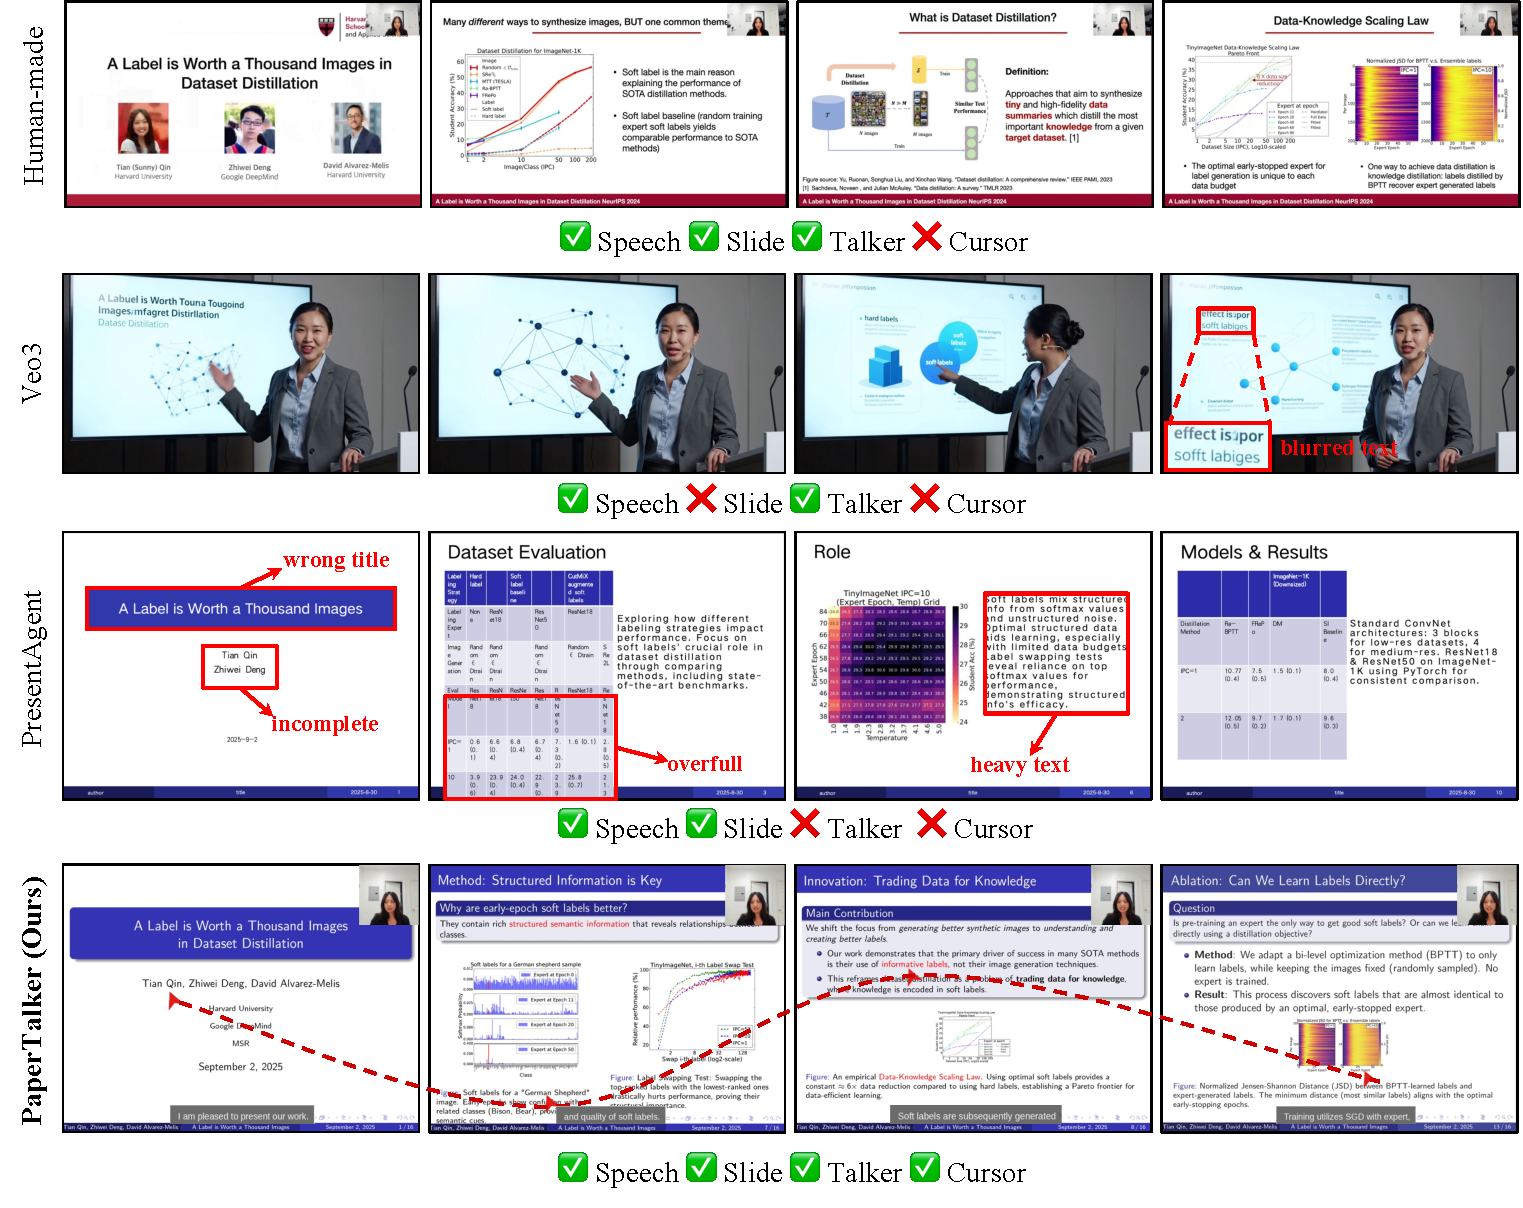
\includegraphics[width=0.95\linewidth]{figure/vis.pdf}
    \vspace{-1\baselineskip}
    \caption{\textbf{Comparison with baselines.} PaperTalker produces slides with rich content, accurate cursor grounding, and an engaging talker, outperforming Veo3 (blurred text, incomplete coverage) and PresentAgent (text-heavy, layout issues, inaccurate info).}
    \label{fig:vis_compare}
  \end{figure}
  \vspace{0.2cm}
  \begin{figure}
    \centering
    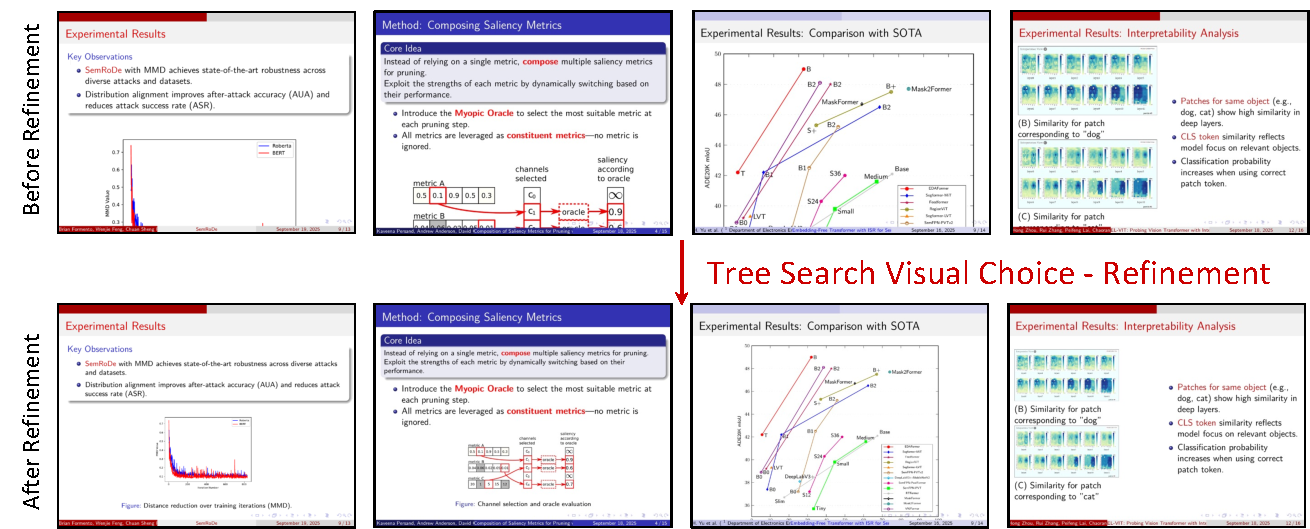
\includegraphics[width=0.95\linewidth]{figure/tree_search_vis.pdf}
    \vspace{-1\baselineskip}
    \caption{\textbf{Effectiveness of Tree Search Visual Choice.} The second row shows slides after refinement, resolving overfull issues from the first row.}
    \label{fig:tree_search_vis_compare}
  \end{figure}
</frame>

% Corresponds to the source text Section 6: Conclusions, and Appendix: Limitations and Future Work
\begin{frame}{Limitations and Future Work}
  % Corresponds to source text Section 6 and Appendix
  \begin{block}{\small Limitations}
   \footnotesize
    \small
    \begin{itemize}
      \item \alertterm{Long-document parsing}: Challenges remain in fully comprehending extremely long and complex papers.
      \item \alertterm{Highly technical equations}: Accurately explaining and integrating complex mathematical formulas within presentation context is difficult for end-to-end generation.
    \end{itemize}
  \end{block}
  \vspace{-0.5\baselineskip}
  \begin{block}{\small Future Research}
   \footnotesize
    \small
    \begin{itemize}
      \item \alertterm{Enhanced semantic understanding} for even longer, more complex papers.
      \item \alertterm{Multilingual support} and advanced accessibility features.
      \item \alertterm{Development of real-time interactive video agents} for tutorials or Q\&A sessions. % Added missing \item
      \item Closed-loop evaluation protocols involving both humans and intelligent audience proxies.
    \end{itemize}
  \end{block}
</frame>

\begin{frame}
  \centering
  \Huge \textbf{Thank You!}
  \vspace{0.7cm}

  
\includegraphics[width=0.15\textwidth]{figure/logo_.png}

  \vspace{0.3cm}
  \large
  \texttt{Questions and Discussion Welcome.} \\
  \href{mailto:e1374425@nus.edu.sg}{e1374425@nus.edu.sg}
\end{frame}
\end{document}